\documentclass[a4paper,11pt]{report}
\usepackage[margin=1in]{geometry}
\usepackage[T1]{fontenc}
\usepackage[utf8]{inputenc}
%\usepackage{lmodern}
\renewcommand{\familydefault}{\sfdefault}
\usepackage{helvet}
\usepackage{pdflscape}
\usepackage{pdfpages}
%\usepackage[latin1]{inputenc}
\setcounter{secnumdepth}{3}

\usepackage[long,nodayofweek]{datetime}
\newdate{date}{12}{09}{2014}

\usepackage{siunitx}
\usepackage[ampersand]{easylist}
\usepackage[inline]{enumitem}
\usepackage{multicol}
   

% % % % % % % % % % Helpers
\usepackage{easy-todo}

% % % % % % % % % % Figure
\usepackage{graphicx,tikz}
\usepackage{caption}
\usepackage{subcaption}
\usetikzlibrary{shapes}
\usepackage{wrapfig}
\graphicspath{ {Images/} }

\usepackage[backend=biber,citestyle=ieee,doi=false,isbn=false]{biblatex} 
\addbibresource{./Bibliography/Thesis.bib}

\AtEveryBibitem{\ifentrytype{misc}{}{
    \clearfield{url}
    \clearfield{urldate}
  }
}

\usepackage[nonumberlist,acronym,toc,shortcuts]{glossaries}
\robustify{\gls}% Make \gls not fragile
\loadglsentries[main]{Abbreviations}
\makeglossaries

% % % % % % % % % % Symbols for footnotes
\renewcommand*{\thefootnote}{\fnsymbol{footnote}}

\usepackage[hidelinks]{hyperref}
\usepackage[all]{hypcap}

% % % % % % % % % %Chapter Title Encoding
\usepackage{titlesec, blindtext, color}	
\definecolor{gray75}{gray}{0.75}
\newcommand{\hsp}{\hspace{10pt}}
\titleformat{\chapter}[hang]{\huge\bfseries}{\thechapter\hsp\textcolor{gray75}{|}\hsp}{0pt}{\LARGE\bfseries}

\begin{document}

\begin{titlepage}
\thispagestyle{empty}
\pagenumbering{gobble}
\begin{center}

  \vspace{.5cm}
  \huge{Comparison of link layer of BLE and 802.15.4}\tiny{}\\
  \vspace{0.3cm}
  \begin{tikzpicture}
	\draw[gray,ultra thick] (0,0) -- (14,0);
  \end{tikzpicture}\\
  \vspace{0.2cm}
  \LARGE{\textit{Running on Contiki OS}}\\
  \vspace{2cm}
  \Large{Master Thesis}\\
  

  \vspace{2cm}		
  \LARGE{PrithviRaj Narendra}
  \vspace{3.5cm} 
  
  \large{\textit{Supervisor}}\\
  \LARGE{Simon Duquennoy}\\
  \vspace{0.2cm}
  \Large{Senior Researcher, SICS}\\
  \vspace{2cm}
  
  \large{\textit{Academic Examiner}}\\
  \LARGE{Mats Brorsson}\\
  \vspace{0.2cm}
  \Large{Professor, KTH}\\
  \vspace{2cm}

\large
EIT ICT Labs Master School Embedded Systems Program\\
School of Information and Communication Technology\\
KTH Royal Institute of Technology\\
Stockholm, Sweden\\
\vspace{1cm}
\displaydate{date}
\\
\end{center} 

\end{titlepage}

\newpage\null\thispagestyle{empty}\newpage

\thispagestyle{plain}
\pagenumbering{roman}
\phantomsection
\addcontentsline{toc}{chapter}{Abstract}
\huge{\textbf{Abstract}} \\
\normalsize \\


There has been extensive research in the low power Wireless Sensor Network (WSN) community with 802.15.4 based platforms. A major factor for this is the support for 802.15.4 based platforms in lightweight Operating Systems (OS) for Internet of Things (IoT) devices. Bluetooth Low Energy (BLE) with its standardized protocol and wide adoption in mobile devices is well suited to all applications requiring direct interaction with a mobile device. BLE does not have support in any of these software platforms for IoT development. With this as motivation this thesis creates a port of Contiki OS to a BLE platform, specifically a platform based on nrf51822 System on Chip (SoC). This will enable direct communication of Contiki nodes with smart-phones and ease development of BLE based projects with Contiki.

This thesis extends the research on BLE by comparing its link layer with 802.15.4's ContikiMAC and Null-RDC on four metrics, namely data rate, latency, reliability and energy consumption. Their behavior with and without external WiFi interference also has been looked into. The tests conducted showcases the performance of simple point to point communication 802.15.4, which is rarely benchmarked in research community that prefers testing complex topologies. The effect of the limits of the number of packets communicated per connection interval in different BLE stacks can be seen on the data rate achievable with BLE. The influence of frequency hopping on the reliability of BLE communication with the presence of external interference is assessed. Adaptive Frequency Hopping (AFH) has been emulated by manually choosing interference free channel map and its effect on mitigating interference has been evaluated. Tests also assesses the impact of BLE link layer configuration, especially creating an asymmetric connection by using non zero slave latency value on latency and energy consumption. With this asymmetric connection, the slave devices have been recorded to a latency of 16 ms with Radio Duty Cycle (RDC) of 0.6\%. %In the same test suite the 802.15.4 queried node had a latency of 24 ms (100\% RDC) and 90 ms (1.3\% RDC) when using Null-RDC and ContikiMAC respectively.



%Internet of Things (IoT) is at the peak of 2014's `Hype Cycle for Emerging Technologies'. Fervent work is being carried out to achieve this vision of billions of interconnected smart devices by researchers, companies and hobbyists. This thesis project focuses on two key technologies fueling the development of IoT devices, namely Bluetooth Low Energy (BLE) and Contiki Operating System (OS). More specifically, this thesis aims to port Contiki OS to a BLE based hardware platform and compare the link layer of BLE with 802.15.4 based Medium Access Control (MAC) layers used in Contiki. 

%The process of porting began with compiling a list of `must have' and `nice to have' requirements for the BLE platform to which Contiki would be ported. An exhaustive list of features of the available platforms was aggregated and based on the requirements identified, the nrf51822 System on Chip (SoC) based platform was chosen. The vendor of this platform provided a BLE stack as a binary, which was used in this project. All the basic features of a Contiki port such as the Contiki clock for etimer, rtimer, serial-line and LEDs have implementations for the chosen platform. \todo{The radio peripheral was left out since it was controlled by the stack in the binary, although an additional task of developing an BLE advertisement packet logger has been done from scratch.} This port has been utilized for a demo application and for the test cases described below.

%The primary research output of this thesis is the comparison of performance of the link layer of BLE with 802.15.4 based ContikiMAC and Null-RDC layers of Contiki in terms of data rate, reliability, latency and energy consumption. Two test suites were designed to collect data of these four metrics and compare the two protocols. Some test cases also included presence of external interference caused by presence of heavy WiFi traffic. The scenario assumed is where one device is unconstrained with respect to availability of power while the other is not.

%In terms of the data rate, the 802.15.4's NullRDC layer achieved the highest at 155 kbps without Clear Channel Assesment (CCA). The effect of WiFi interference overlapping in the channel of communication in case 802.15.4 can be seen when the data rate reduced to 61 kbps from 148 kbps in the case where interference was in a different channel. With 802.15.4 the data rate can be maximized by having Radio Duty Cycle (RDC) of 100\%. The influence of frequency hopping in BLE can be noticed when the data rate decreased to only 23 kbps from 29 kbps when WiFi interference was introduced, both cases having RDC of around 27\%.  In BLE the effect of packets communicated per connection interval can be seen when communicating with an Android device as the data rate increased to 86 kbps, in which RDC was 44\%. 

%Use of 802.15.4's CCA delivered a Packet Reception Ratio (PRR) of 99\% and 79\% with and without WiFi interference respectively. In case of BLE, the link layer's the simple acknowledgment scheme achieved a Packet Delivery Ratio (PDR) of 100\%. Without WiFi interference, BLE achieved a PRR of almost 100\%. When WiFi interference was introduced, PRR resurged back to greater than 99\% when WiFi free channel map was used as compared to 80\% when complete channel map, which shows working of Adaptive Frequency Hopping (AFH).

%802.15.4's latency was measured as 24 ms with Null-RDC and 90 ms with ContikiMAC. With BLE latency values ranging from 14 ms to 750 ms were observed. These tests to measure latency show the influence of link layer parameters such as `connection interval' and `slave latency', as well as whether the data is queried by the master node or the slave node. The change in symmetry of the connection with non-zero slave latency can be seen in case where the latency changes from 16 ms to 736 ms when the test case changes from the slave querying the data to the master querying the data. The master's RDC of 22\% and slave's RDC of 0.6\% also indicates the asymmetry in the connection. With these different configurations, the different use cases are also illustrated.

\clearpage

%\newpage\null\thispagestyle{empty}\newpage
%
%\thispagestyle{plain}
%\phantomsection
%\addcontentsline{toc}{chapter}{Sammanfattning}
%\huge{\textbf{Sammanfattning}} \\
%\normalsize \\
%Hello Sammanfattning.
%\clearpage

\newpage\null\thispagestyle{empty}\newpage

\thispagestyle{plain}
\phantomsection
\addcontentsline{toc}{chapter}{Acknowledgment}
\huge{\textbf{Acknowledgment}} \\
\normalsize \\


Foremost I would like to earnestly thank my supervisor at Swedish Institute of Computer Science (SICS), Simon Duquennoy, for agreeing to supervise me in a topic that I proposed, guiding me patiently, consistently reviewing and providing constructive feedback for my work. Next I would like to thank Thiemo Voigt and the Networked Embedded Systems group at SICS for their warm inclusiveness and assisting me whenever I needed help. As usual this open source work stands on the shoulders of giants, I'm thankful for their amazing work. For all the resources and guidance that I have received in various forms from my fellow netizens, I'm grateful to them. I thank EIT ICT Labs for believing in me and providing me this opportunity. As always, my family and friends have supported and encouraged me, and for that they have my heartfelt thanks.
\clearpage

\newpage\null\thispagestyle{empty}\newpage

\tableofcontents
\null
\vfill
\begin{wrapfigure}{r}{0.25\textwidth}
\vspace{-30pt}
  \begin{center}
	\includegraphics[width=0.22\textwidth]{cc-by}
  \end{center}
\end{wrapfigure}
\noindent
{\large This work is licensed under a \href{http://creativecommons.org/licenses/by/4.0/}{Creative Commons Attribution 4.0 International License}.}


\glsnogroupskiptrue
\renewcommand{\glsnamefont}[1]{\textbf{#1}}
\setlength{\glsdescwidth}{0.8\hsize}
\printglossary[style=long,title=List of Abbreviations,type=\acronymtype]
\clearpage

\addcontentsline{toc}{chapter}{\listfigurename}
\listoffigures
\clearpage
\addcontentsline{toc}{chapter}{\listtablename}
\listoftables
\clearpage

\pagenumbering{arabic}
\chapter{Introduction}

\section{General introduction to the domain of the thesis}

What is \gls{ble}? Why was it developed and who/where is it being used?  \cite{Gomez2012}

What is Contiki \gls{os}? Why was it and who/where is it being used? Explain the amount of R\&D done in terms of communication protocols based on 802.15.4 \cite{Contiki}.


\section{Problem definition}
Need for \gls{ble} in Contiki as a platform for \gls{iot}. To understand the characteristics of \gls{ble} and 802.15.4 so that we can identify the applications suitable for these protocols.

\section{Goal}
To choose and integrate a \gls{ble} hardware platform with Contiki. To compare \gls{ble} and 802 in various performance criteria of data-rate, latency, reliability and energy consumption in environments with and without external interference.

\section{Outline of the report}

\todo{method??}
\chapter[Background]{Background\footnote{Includes text and images from minor thesis 'Business ideation for \gls{ble}'}}

\section{Overview of \acrlong{ble}}
Rest of overview, from what is missed in 1st chapter.

\subsection{Design objectives of \gls{ble}}
\gls{ble} was designed by Bluetooth \gls{sig} from the ground up, which helped it achieve certain design goals. These design goals for this wireless personal area network were \emph{low cost, worldwide operation, short range, robustness} and \emph{low power}\cite{Heydon2012}. 
\paragraph{Low Power} \gls{ble} aims to use a tiny batteries such as button cell to keep a device operating for months to years. To achieve this goal, \gls{ble} was optimized to communicate small amounts of data, such as the states of devices. Also \gls{ble} is optimized to have lower peak power requirements, which allows use of button cells to be used with \gls{ble} devices.
\paragraph{Worldwide Operation}
For a technology to be adopted, it is important that there is uniform conformity to the regulations around the world. The 2.4 \si{\GHz} \gls{ism} radio band is the only one available license free worldwide. The technology to develop wireless devices in this band is mature making it the suitable radio band for \gls{ble}.
\paragraph{Short Range}
\gls{ble} was designed to be for personal area network like Classic Bluetooth, which means that it is not a network to work with a cellular base station network. This design criterion goes hand in hand with \emph{low power}.
\paragraph{Low Cost} Lower power requirements mean that the batteries in \gls{ble} devices need to smaller and have to be replaced less frequently, both resulting in a reduction of cost for both the manufacturer and the customer. The use of the \gls{ism} band for communication levels removes the licensing entry barrier for start-ups to develop \gls{ble} devices. \gls{ble} embraces simplicity in its pursuit to lower the cost. \gls{ble} supports only single-hop communication in a star network, which reduces the memory and processor requirement for supporting the protocol. Simplicity was the key factor for the choosing of \gls{gfsk} as the modulation scheme for \gls{ble} to result in low cost, small radio implementation of the radio in the \glspl{ic} for \gls{ble}. 
\paragraph{Robustness} The 2.4~\si{\GHz} space is crowded with devices communicating with various standards as well as spurious noise making the robustness a key criteria in developing \gls{ble} standard. \gls{ble} uses a multi-channel hopping mechanism called \gls{afh} to detect, avoid and recover from interference. In addition to \gls{afh}, \gls{ble} uses \gls{crc} to detect and recover from bit-errors due to background noise.

\subsection{\gls{ble} network architecture}
Single and Dual devices,
Advertisers and scanners,
Master and Slave,
Star Network,
figure \ref{devicesBLE}
\begin{figure}[h] %{r}{0.51\textwidth}
%\vspace{-15pt}
  \begin{center}
	\includegraphics[width=0.49\textwidth]{devicesBLE}
  \end{center}
\caption{Typical BLE network}
%\vspace{-10pt}
\label{devicesBLE}
\end{figure}

\section{\gls{ble} stack overview}
Explain host and controller division. More details about \gls{ll}.

\textbf{Image of the stack}

\paragraph{Physical layer}
\paragraph{\acrfull{ll}}
\paragraph{\gls{l2cap}}
\paragraph{\gls{gap}}
\paragraph{\gls{att}}
\paragraph{\gls{gatt}}
\paragraph{\gls{sm}}

\section{Overview of Contiki}
??????????????? Which aspects of Contiki here?

\section{Overview of 802.15.4}
Mention that in this thesis the Contiki specific implementations of the 802.15.4 layers will be tested.

\subsection{Physical layer}

\subsection{\gls{mac} layer}
\subsubsection{\gls{rdc} layer}
\subsubsection{\gls{csma}}

\todo{Seperate section Previous work done on comparing \gls{ble} and 802.15.4}



\chapter{Methodology}

\section{Research process}

Figure \ref{RePrSteps} shows tasks performed in this thesis boxes of the flow-chart and the steps of the research process on the left. The thesis report is also organized in this manner.

\begin{figure}[h]
\centering
\def\svgwidth{0.93\columnwidth}
\input{./Images/RePR.pdf_tex}
\vspace{-10pt}
\caption{Thesis' tasks and steps in the research process}
\label{RePrSteps}
\end{figure}

\section{Research Method}

In this experimental research large amount of data was generated to compare the two protocols mentioned, hence utilizing quantitative research method. The approach followed was deductive as the experiment started by defining the metric to measure, then designing the test to perform and finally deducting the conclusions based on the collected data from the tests.

The data collected was condensed with descriptive statistics and graphical representation was used to showcase this information. Univariate analysis  of the various metrics of the two protocols was compare the two protocols from these graphical representation.
\chapter{Literature Study}

\section{Porting Contiki \gls{os} to a new platform}
Contiki \gls{os} project originating in 2002 has been ported to an increasing number of hardware platforms\cite{contikiHw}. Since Contiki is an open-source BSD Clause-3 licensed project, there are many projects in various hardware platforms based on a fork from the Contiki repository.

These hardware platforms' processors range across a spectrum of 8-bit (8051 and AVR), 16-bit (MSP430) to 32-bit (ARM Cortex-M, PIC32). Contiki has support for 802.15.4 based wireless communication with various external transceivers and \glspl{soc} with built in radio transceiver. Various common features of many platforms such as \glspl{led}, buttons and serial port have modules in Contiki for common \gls{api} across platforms.

In \cite{Oikonomou2011} the authors describe Contiki's port to a CC2430 based platform manufactured by Sensinode Ltd. CC2430 is an enhanced Intel 8051 processor based \gls{soc} having 802.15.4 physical layer compatible radio transceiver. The authors fully debugged the port which had of a code footprint of about 100 \gls{kb}, varying based on the compiler mode and the features enabled. Many new features were added to the port including support for \gls{adc} unit, all the sensor available on the platform (accelerometer, light sensor, voltage and temperature sensors), watchdog timer and the general purpose buttons. Because of the limited stack availability of 233 bytes, many optimizations such as moving variables to external \gls{ram} memory space and re-writing the radio driver for CC2430 to prevent stack from overflowing.

Contiki was ported to two new platforms, namely MicaZ and TelosB in a Bachelor thesis \cite{stan2007porting}. TelosB, similar to the TMote-Sky platform, consists of a 8MHz 16-bit MSP430 \gls{mcu}, a CC2400 transceiver with 802.15.4 \gls{phy} and a host of sensors to measure light, temperature and humidity. The port to TelosB was done by changing the port to the fully supported TMote-Sky platform. MicaZ platform consisted of a 8-bit Atmel ATMega128L \gls{mcu} and a CC2400 transceiver. MicaZ platform needed rewriting of the code for processor abstraction so that the high level Contiki \glspl{api} could work.

Contiki has been ported into platform based on a ARM Cortex M3 processor to create a device wired with Ethernet to connected to the Internet \cite{Wilde2013a}. Ethernet based networking with the libraries present in Contiki was developed in this project to demonstrate as a proof of concept.

There are many unofficial ports of Contiki to various hardware platforms, including ones based on ARM Cortex M3 based processors. This can be seen in the port to STM32F10x based platform \cite{Padrah} and LPC1768 based platform \cite{Tanyingyong2013}, both having Cortex M3 processor.

\section{Evaluating the performance of \gls{ble}}
In a paper \cite{Gomez2012} providing an overview and evaluation of \gls{ble}, its various parameters such as energy consumption, latency, maximum piconet size and throughput have been evaluated. Theoretical calculations were done to predict the lifetime of a \gls{ble} slave device running of a 230 mAh coin cell battery for different values of \emph{connection interval} and \emph{slave latency}. The average current consumption of a TI CC2540 \gls{ble} platform was plotted for the entire range of connection interval keeping the slave latency as zero. The estimate of the lifetime was also done with respect to various \gls{ber}.

\todo{Talk about latency wrt Gomez2012}
The same experimental setup \cite{Gomez2012} shows the maximum throughput between two CC2540 devices as 58.48 kbps. This is attributed to the fact that in each connection event with an interval of 7.5 ms four packets are not transmitted as in an ideal case. An analytical model of the throughput \cite{Gomez2011} has been developed for different \gls{ber} and connection interval. Simulation results validate this model developed.

The energy consumption for an advertiser and scanner is modeled for the activity of the scanner discovering the advertiser \cite{liu2012energy}. The current consumption for each phase of advertisement and scanning is measured. Using this information the a model of the energy consumption is developed taking into account the advertising and scanning interval. The model developed is compared with experiments and validated. 





Energy \cite{Kindt2014} \cite{liu2012energy}

Throughput, Energy
\todo{decode whats said in Mackensen2012}
\cite{Mackensen2012}


\section{Evaluating the performance of 802.15.4}

\section{Comparison of BLE and 802.15.4}

Low power\cite{Siekkinen2012} SimpliciTI\cite{Mikhaylov2013} ZigbeeANT \cite{Dementyev2013}

\chapter{Porting a \gls{ble} platform to Contiki \gls{os}} \label{5bleContiki}

This chapter describes the initial task of choosing the hardware platform supporting \gls{ble} and porting Contiki \gls{os} to this platform. This task was a pre-requisite to the next task of testing detailed in chapter \ref{6Testing}. Section \ref{5HwPlt} explains the process of choosing a hardware platform and describes the chosen one. Section \ref{5Porting} describes the different aspects of porting Contiki to a new platform, with details of the specific port done in this project.

\section{\gls{ble} Hardware Platform} \label{5HwPlt}

As mentioned in section \ref{4Porting} Contiki has been ported to many hardware platforms. Since one of the main feature of Contiki is its communication stack capable of running in resource constrained systems, the primary aspect of a hardware platform is the \gls{mcu} and the communication interface. When choosing a hardware platform there are many other aspects that need to be considered as well. These include the availability of source code for peripheral drivers and examples, development environment (compiler, linker, programmer and debugger), development boards, documentation of the entire system and online forum for discussion.

Before this project, Contiki only supported wireless communication based on 802.15.4 physical layer. There are two types of platforms, namely platforms which consist of a discrete radio transceiver with a \gls{mcu} controlling it and platforms which consist of a \gls{soc} containing both the \gls{mcu} and radio transceiver in the same \gls{ic}. For including \gls{ble} support in Contiki, a hardware platform needed to be chosen and this process is explained in this section.

\subsection{Requirements of the hardware platform}
The \emph{mandatory} requirements for the platform would be:
\vspace{5pt}
\begin{easylist}[itemize]
& A \gls{soc} based platform.
& Must have a well supported and documented processor with good specifications.
& For a open source project such as Contiki, a free (and preferably open source) development toolchain must support the platform.
& Availability of well documented datasheet and user manual.
& Availability of an evaluation/development kit.
& Enough memory to accommodate Contiki and \gls{ble} stack’s requirements.
& Presence of basic peripherals such as timers and serial port required for Contiki.
\end{easylist}
\vspace{10pt}
\noindent
The non-mandatory, although \emph{nice to have} requirements for the platform would be:
\vspace{5pt}
\begin{easylist}[itemize]
& Presence of flexible power modes with low active and sleep power consumption.
& Availability of a good set of peripherals.
& Availability of \gls{ble} stack from the vendor, preferably with source code.
\end{easylist}
\vspace{10pt}

\subsection{Comparison and selection of the hardware platform}

With these requirements, based on the exhaustive comparison in \hyperref[AppendixA]{Appendix A} of the available \gls{soc} (\gls{ble}+\gls{mcu}) solutions available today, a platform based on nRF51822 from Nordic-Semiconductors would be a suitable option. As seen from the table in \hyperref[AppendixA]{Appendix A}, this platform would satisfy all the requirements mentioned above except for that the \gls{ble} stack would be available as a binary file, without the source code.

As shown in the table in \hyperref[AppendixA]{Appendix A}, recently many new promising \gls{ble} based \glspl{soc} have be released such as Quintic 9020, Dialog Semiconductor DA14580, Lapis MLA7105 and Broadcom BCM20732. From the limited technical information available about them, their technical specifications would be suitable for a project like this. But because of the limited documentation about them, scarce availability and nascent support they are not suitable.

\subsection{Overview of nrf51822 \gls{soc} and its platform} \label{5nrfPCA}

nrf51822 is a \gls{soc} made by Nordic Semiconductor for developing \gls{ble} and 2.4 GHz based wireless systems \cite{nrf51822page}. Most of the specification of this \gls{soc} can be found in the table in \hyperref[AppendixA]{Appendix A}. The ARM Cortex M0 present is a 32 bit, 3 stage pipeline processor with Von Neumann architecture. It is designed for low silicon die size, low cost and power. It has an integrated \gls{nvic}  responsible for handling processor exceptions and peripheral interrupts. 

The development boards in the form of a USB dongle used for this thesis are called PCA10000. As seen in the figure \ref{pca10000}, the top side of PCA10000 contains nrf51822 at the centre, powered from the USB port through a voltage regulator. This \gls{soc} is connected to a tri-colour RGB led, a 16 MHz crystal, a 32.768  kHz crystal and a PCB antenna with its matching network. On the other side of the PCB is the SEGGER JLink Lite Cortex M unit. This can program and debug using the Serial Wire Debug (SWD) port of nrf51822. Another useful feature of this board is that the SEGGER JLink unit provides a serial port over USB with hardware flow control (HWFC) to the computer that this dongle is connected to. This serial port is connected to the \gls{uart} port of nrf51822 \cite{PrithviR}.

\begin{figure}[h]
\includegraphics[width=\textwidth]{PCA10000}
\caption{PCA10000 development board}
\label{pca10000}
\end{figure} 

Nordic Semiconductor provides \gls{ble} stack as a precompiled and linked binary file called \emph{SoftDevices}. The SoftDevice is stored in a protected area in the flash memory and has access to a protected section of \gls{ram} memory, preventing unauthorized access by the application code. The SoftDevice can be accessed through a specified set of \gls{api} calls. These \glspl{api} are accessed by making a supervisor call to the processor causing a exception handler to run the SoftDevice. All calls are non-blocking, which means that the call will not stall the application making the call. And there are synchronous and non-synchronous calls, where the synchronous calls immediately return the result while the asynchronous calls start an operation that will send the result as an event to the application. The SoftDevice is used for accessing the \gls{ble} stack as it was out of the scope of this thesis project to implement a \gls{ble} stack from scratch.

A \gls{sdk} is provided for nrf51822 which contains the peripheral drivers, examples, the interface header files for the SoftDevices and their documentation. Two tools provided by Nordic Semiconductor has been extensively used in this thesis. \emph{nRF Sniffer} is a tool used with the PCA10000 board and \emph{Wireshark} application to capture, view and save the information of \gls{ble} packets being sent between two devices. This greatly helps in learning about \gls{ble} packets and debugging problems. This tool is capable of providing detailed information about almost all the segments of the captured packets. It was found in during the thesis project that the nRF-Sniffer is not entirely capable of capture each and every packet being communicated, which does limit its use as tool to get feedback as one develops low level \gls{ble} drivers. Another invaluable tool provided by Nordic Semiconductor is \emph{Master Control Panel}. It is an Android application which acts a generic \gls{ble} application capable of discovering \gls{ble} devices, connect and communicate with them while providing an overview of their Attribute database. 

From actively using this platform for many months, the subjective pros and cons of this platform are stated below.

\noindent Pros:
\begin{easylist}[itemize]
& Large, mature and active community
& Support of open-source Eclipse and GNU-GCC development environment 
& Availability at low price
& Cortex M0 processor with competitive specs
& Support in mbed, an online open source development platform
& Support of supplementary tools such as nRF-Sniffer and android application 'Master Control Panel'
\end{easylist}
\vspace{5 pt} \noindent Cons:
\begin{easylist}[itemize]
& The \gls{ble} stack available as binary reducing flexibility
& \gls{sdk} not open for distribution
\end{easylist}

\section[Porting PCA10000 platform of nrf51822 to Contiki]{Porting PCA10000 platform of nrf51822 to Contiki\footnote{Available at \url{https://github.com/EarthLord/contiki} with complete Doxygen documentation}} \label{5Porting}

\subsection{Development Setup}
Contiki was initially developed in a Linux based operating system, although Windows is also supported now. The porting of PCA10000 platform to Contiki was done in Ubuntu 13.10 and 14.04. The compiler suite used is GNU Tools for ARM Embedded Processors Version 4.8.3. The program used for programming the binary files compiled was SEGGER J-Link Commander V4.90 using the Segger JLink programmer on PCA10000. The front end used to write the code is the Eclipse IDE for C/C++ Developers Version Kepler Service Release 1 and Sublime Text.

\subsection{Folder structure of Contiki}
When porting a new platform to Contiki, the three folders inside a Contiki distribution where additions need to be made are cpu, examples and platform. The content in these folders are as described below. The location of the Contiki distribution is represented by the path `CONIKI'. The port of nrf51822 \gls{soc} with its PCA10000 board also follows this convention.

\paragraph{CONTIKI/cpu}In this folder, all the files contain implementation which is solely dependent on the \gls{soc} is present. This includes the code for the processor abstraction, the drivers of the peripherals of the \gls{soc}, makefile with commands for compiling and linking the code, linker file and the documentation of these implementation. The boot-loader  or start-up code, if required is also present here. The peripheral drivers for peripherals such as timers and serial port must use the \gls{api} format of Contiki so that the libraries of Contiki using these peripherals can operate correctly. The exact implementations of these drivers is explained in section \ref{peripheralsContiki}. 

\paragraph{CONTIKI/platform} An \gls{soc} over time has increasing number of boards or systems that are based on it and these are referred as platforms in this folder. Every board has its own folder in this platform folder which contains files which contain implementation which is dependant on the particular board. These include the specification of the connections to the LEDs, buttons, sensors and serial ports, power sources, the clock sources, memories present and any other board specific details. Any peripheral driver implementation specific to the board is present here. The default project specifications such as the source and frequency of clock and serial baud-rate are defined here. The main function where the execution of the program starts and initialization of all the peripherals and libraries used by Contiki happens is present here.

\paragraph{CONTIKI/examples} The examples folder contains all the files related to projects that are implemented using Contiki with any of the supported hardware platforms. The makefile where the make command is executed is present here. The compiled object and binary files are also stored here. The default specifications of the platform can be overridden by creating a \texttt{project-conf.h} in the specific example.

\subsection{Peripherals required for Contiki}\label{peripheralsContiki}
\paragraph{Contiki clock}
Contiki clock, which is the source for all the timers, except the rtimer, is provided by the RTC1 peripheral of nrf51822. RTC1 is chosen because when a SoftDevice is used, RTC0 will not be accessible for the user application. The \gls{rtc} peripheral uses the \gls{lfclk} of nrf51822, which can be generated by a crystal or RC oscillator to produce 32.768 kHz. For Contiki clock, there are two implementations made, namely Tickless and Ticks which are described below. 

\subparagraph{Ticks}
For this implementation the RTC1 peripheral is configured such that an interrupt is called for its every increment or \emph{tick}, hence the name. This happens at 64 Hz, which is the default value of \texttt{CLOCK\_SECOND}. In the interrupt routine, the current clock tick is incremented, an etimer poll is requested if an etimer has expired and every \texttt{CLOCK\_SECOND}\textsuperscript{th} interrupt the second count is incremented. The variable storing the clock `ticks' and `seconds' is returned upon their request from any other process.

\subparagraph{Tickless}
In this implementation, the processor will not be woken up at every tick of the \gls{rtc} peripheral, hence the name. To enable this, a small addition is required to the etimer and clock module present at \texttt{CONTIKI/core/sys}. Every time the next etimer expiration is computed, the clock module is informed of it. With this additional information the \gls{rtc} can configure a compare interrupt to poll the etimer upon its expiry. The RTC1 peripheral is also configured to provide an interrupt only on its overflow so that it can be accounted for when calculating the seconds elapsed. For the 24-bit timer of RTC1, with \texttt{CLOCK\_SECOND} as 64, the overflow interrupt would happen only once every $(2^{24}/64)$ second, that is almost every three days as compared to interrupt happening few times a second in the `Ticks' case. 

With a Tickless implementation, both keeping track of the value of `clock ticks' and polling the etimer upon its expiry is handled by the \gls{rtc} peripheral rather than the processor, which would significantly reduce the power consumption without sacrificing any performance. The only additional development task is the addition in the core Contiki library as mentioned above.

\paragraph{Rtimer}
An rtimer is implemented in Contiki's port to nrf51822 by using the \emph{TIMER1} peripheral, which runs on the \gls{hfclk} of 16 MHz. TIMER1 was chosen as TIMER0 is required by SoftDevice, in case it is used. Since RTimer is required with higher granularity than Contiki Clock, rtimer increments at rate of 62.5 kHz in its current implementation, which is every 16 \si{\micro \second}. This is achieved by TIMER1 is configured as a 8-bit timer providing an interrupt on overflow where the rtimer count is incremented. In the interrupt routine there is also a check to see if the scheduled rtimer task needs to be run by comparing the current rtimer count. It should be noted that Rtimer being run by TIMER1 peripheral requires the \gls{hfclk} to be active, consuming power.

\paragraph{\glspl{led}}
The PCA10000 board has a RGB \gls{led} unit on it. The port allows it to be controlled by the Contiki \gls{api}. This is done through reading and writing to the \gls{gpio} port when the \gls{led}'s status is read and \gls{led}'s state is changed respectively. This implementation is present in \texttt{CONTIKI/platform/dev/led-arch.c} file since the \glspl{led} are not a property of the nrf51822 \gls{soc} but the PCA10000 platform.

\paragraph{Button(s)}
The PCA10000 board does not have any buttons. In case of porting a platform with physical buttons, its implementation would be in the same location as the \glspl{led} i.e. the platform folder.

\paragraph{Serial Port}
The port of Contiki to PCA10000 platform offers abstraction of the \gls{uart} peripheral of nrf51822, which will communicate with the serial port of the computer to which PCA10000 is connected to. Writing to the serial port is achieved by using the \texttt{printf()} function present in the \texttt{stdio.h} library by redirecting \texttt{printf} call's character stream to the \gls{uart} peripheral. Instead of the default NewLib library, the Newlib-nano library is used so that the amount of memory required is reduced.

For receiving the data from the the \emph{serial-line} module of Contiki is used. This module broadcasts an event when a series of characters are received ending with a `newline' (\textbackslash n) character. To use this module, it is initialized on boot and all the characters received by the \gls{uart} port is sent to this module in the \gls{uart} receive interrupt routine.

\paragraph{Radio}
Since the radio peripheral is completely controlled by the SoftDevice for implementing the \gls{ble} stack, it is untouched in this port. To use the radio peripheral, the \glspl{api} provided by the SoftDevice is used.

\subsection{Makefile structure of Contiki}

\textbf{Introduction to makefile and include.}
There are multiple makefiles present across different folders that are included in the way shown in figure \ref{MakefileLevel} to form the complete makefile. In the most basic form these are the makefile in the example folder, `makefile.include' in the Contiki root folder, `makefile.TARGET' in the specific platform folder and `makefile.CPU' in the specific cpu folder, where TARGET and CPU are specific to the project. The port of Contiki to nrf51822's platform follows this convention too.

\begin{figure}[h]
\centering
\def\svgwidth{0.93\columnwidth}
\input{./Images/MakefileLevel.pdf_tex}
\vspace{-10pt}
\caption{Structure of Makefile inclusion in Contiki \gls{os} to form an example specific one}
\label{MakefileLevel}
\end{figure}

%Makefile where the project is present i.e. in the example folder
%-Makefile indicating the target platform (if not already specified)
%-Makefile.include in root CONTIKI directory
%--Makefile of applications, if any are required
%--Makefile of the target, present in the platform directory
%---Makefile of the \gls{soc}, present in the cpu directory

The makefile in the project specific example folder, the different project source files are specified and the `makefile.include' present in the root CONTIKI folder is added. `makefile.inlcude' glues together all the required components of Contiki and provides the default implementation of compiling and linking. The target makefile in the specific platform directory is included here. In `makefile.TARGET' the source files present in this directory are added, any Contiki modules required are added and the \gls{soc} or \gls{mcu} makefile in the specific directory is added. The \gls{soc} or \gls{mcu} makefile adds all the source files present in the CPU directory, specifies the command for compiling the code, linking the objects generated, uploading the executable binary or hex file.

The makefile in the example folder is where the make command is called. The operations that can be performed with this make command depends on the makefile. Usually the operations are cleaning (removing the object and binary files), compiling the source files into object files , linking these object files to create an executable file, creating a binary file from this executable file, uploading the binary to the \gls{soc} to start execution and so on. For the nrf51822 \gls{soc} additional operations of uploading the SoftDevice and erasing the flash are supported.


\chapter{Test Cases}

\section{Performance Metrics Definition}

\paragraph{Data Rate}

\paragraph{Latency}

\paragraph{Reliability}

\paragraph{Energy Consumption}

\section{Data Dump Test Design}

\begin{figure}[h]
    \centering
    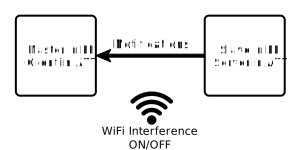
\includegraphics[width=\textwidth]{DataRateSetup}
	\caption{Setup to measure data rate with \gls{ble}}
    \label{fig:DataRateSetup}
\end{figure}

\begin{easylist}[itemize]
& Send packets of maximum size for one minute in the fastest way possible
&& Do one test without CCA for 802.15.4
& Repeat with WiFi
&& Choose a channel interfered by WiFi for 802.15.4 and one channel without WiFi interference.
&& For \gls{ble} do this with channel map with all channels and channel map with WiFi free channels.
& Do this test 10 times
\end{easylist}
\vspace{10pt}


In this test, to measure the various performance criteria in an environment with interference, WiFi interference will be introduced using the tool 'iperf'. The interference pattern generated will simulate streaming of large data over WiFi. \todo{Explain the exact configuration of UDP packets sent}

\vspace{10pt}
Metrics evaluated
\begin{easylist}[itemize]
& Data Rate
& Reliability
& Energy Consumption
\end{easylist}

\section{Request Response Test Design}

\begin{easylist}[itemize]
& Explain what is meant by request response
& Different cases in \gls{ble} and 802.15.4
\end{easylist}

Metrics evaluated
\begin{easylist}[itemize]
& Latency
& Energy Consumption
\end{easylist}


\pagebreak

The objectives of the tests are to compare the link layer of \gls{ble} and 802.15.4 in the aspects mentioned in the following sections. 

The \gls{ll} of 802.15.4 consists of \gls{mac} layer on top of a \gls{rdc} layer. For the RDC layer the Null-RDC and ContikiMAC driver will be tested in each of the test with \gls{csma} as the \gls{mac} layer. In case of Contiki-MAC the receiving node switches on periodically to sense if there are any packets that need to be received. The default time of this period is 125 ms. In case of null-RDC the radio receiver is never switched off, as the name suggests.

For \gls{ble}, communication will be done at the Generic Attribute (GATT) layer because the binary from Nordic Semiconductor used in this project does not provide APIs to access the lower layers in both peripheral and central devices. In all the tests the packet structure in 802.15.4 will be same as in \gls{ble} above the link layer.
In this test, to measure the various performance criteria in an environment with interference, WiFi interference will be introduced using the tool 'iperf'. The interference pattern generated will simulate streaming of large data over WiFi. \todo{Explain the exact configuration of UDP packets sent}
In \gls{ble}, the devices can assume different roles in the different layers of the protocol. In the \gls{ll} a device can be a 'Master' or a 'Slave'. In the \gls{att} layer, a device can be a 'Client' and/or 'Server'. A server contains data and the client can request data from the server.

In some of the tests, to measure the various performance criteria in an environment with interference, WiFi interference will be introduced using the tool 'iperf'. The interference pattern generated will simulate streaming of large data over WiFi.

\section{Data Rate Test}
This experiment aims to measure the maximum data rate of \gls{ble} and 802.15.4 at the LL with and without WiFi interference. For the \gls{ble} test the devices are configured as shown in the diagram below.

\begin{figure}[h]
    \centering
    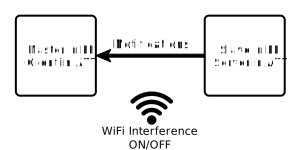
\includegraphics[width=\textwidth]{DataRateSetup}
	\caption{Setup to measure data rate with \gls{ble}}
    %\label{fig:DataRateSetup}
\end{figure}

In this test the data rate is measured by sending data from the server to the client which is not acknowledged in the \gls{att} layer. The data rate is measured at the receiver i.e the Master device. The packet structure will be used such that the complete packet size of \gls{ble} is used. Each run of the test will last of one minute to collect enough data to measure the average data rate.

In case of 802.15.4 one node is configured as transmitter and the other as receiver. The data-rate will be measured at the receiver. In these tests two channels will be used, one which interferes with WiFi and one which does not. This means that each channel will be tested with and without interference. The complete packet size of 802.15.4 will be used when conducting this test.

For data rate measurement tests in both the standards with and without WiFi, the data rate will be measured by sending data for one minute. The data rate will be expressed in both packets per second and \gls{kbps}. 

\subsection{Latency}
This experiment aims to measure the latency for a read request in case of \gls{ble} and 802.15.4, i.e. the time difference between sending the read request packet and receiving the packet with the value requested. In case of both the protocols there are intervals at which the radio is active, where communication can take place. To make sure that the read request packets are sent randomly at any point in this interval, timers with random values would be used to initiate sending these packets. The table below shows the connection parameters used for the various tests to measure the latency with \gls{ble}. The latency is measured at the device sending the packet '1' in the 'Packet' column and is defined as the time from sending the packet '1' to receiving the packet '2'.

\todo{Redo the correct table}


\begin{table}[htbp]
\begin{center}
\begin{tabular}{|l|l|l|l|l|}
\hline
\multicolumn{ 1}{|c|}{\textbf{Connection}} & \multicolumn{ 1}{c|}{\textbf{Connection}} & \multicolumn{ 3}{c|}{\textbf{Devices' Configuration}} \\ \cline{ 3- 5}
\multicolumn{ 1}{|c|}{\textbf{Interval}} & \multicolumn{ 1}{c|}{\textbf{Configuration}} & \multicolumn{ 1}{c}{\textbf{LL}} & \multicolumn{ 1}{|c}{\textbf{GATT}} & \multicolumn{ 1}{|c|}{\textbf{Packet}} \\ \hline
\multicolumn{ 1}{|c|}{} & \multicolumn{ 1}{l|}{Slave latency = 0} & Master & Client & 1. Read request \\ \cline{ 3- 5}
\multicolumn{ 1}{|l|}{} & \multicolumn{ 1}{l|}{
Supervision timeout = 1 \si{\second}} & Slave & Server & 2. Read response \\ \cline{ 2- 5}
\multicolumn{ 1}{|c|}{7.5 \si{\milli\second}} & \multicolumn{ 1}{l|}{Slave latency = 120
} & Master & Client & 1. Read request \\ \cline{ 3- 5}
\multicolumn{ 1}{|l|}{} & \multicolumn{ 1}{l|}{Supervision timeout = 1 \si{\second}} & Slave & Server & 2. Read response \\ \cline{ 2- 5}
\multicolumn{ 1}{|l|}{} & \multicolumn{ 1}{l|}{Slave latency = 120
} & Slave & Server & 1. Indication \\ \cline{ 3- 5}
\multicolumn{ 1}{|l|}{} & \multicolumn{ 1}{l|}{Supervision timeout = 1 \si{\second}} & Master & Client & 2. Indication ACK \\ \hline
\multicolumn{ 1}{|c|}{} & \multicolumn{ 1}{l|}{Slave latency = 0
} & Master & Client & 1. Read request \\ \cline{ 3- 5}
\multicolumn{ 1}{|l|}{} & \multicolumn{ 1}{l|}{Supervision timeout = 1 \si{\second}} & Slave & Server & 2. Read response \\ \cline{ 2- 5}
\multicolumn{ 1}{|c|}{125 \si{\milli\second}} & \multicolumn{ 1}{l|}{Slave latency = 15
} & Master & Client & 1. Read request \\ \cline{ 3- 5}
\multicolumn{ 1}{|l|}{} & \multicolumn{ 1}{l|}{Supervision timeout = 3 \si{\second}} & Slave & Server & 2. Read response \\ \cline{ 2- 5}
\multicolumn{ 1}{|l|}{} & \multicolumn{ 1}{l|}{Slave latency = 15
} & Slave & Server & 1. Indication \\ \cline{ 3- 5}
\multicolumn{ 1}{|l|}{} & \multicolumn{ 1}{l|}{Supervision timeout = 3 \si{\second}} & Master & Client & 2. Indication ACK \\ \hline
\end{tabular}
\end{center}
\caption{\gls{ble} latency measurement test cases}
\label{tbl:testcases}
\end{table}

Where,

\emph{Connection Interval}: After a \gls{ble} connection is established, the master device must always send a packet to the slave periodically after the time specified in connection interval. These connection events provide an opportunity for the slave to communicate with the master.

\emph{Slave Latency}: The maximum number of connection events that a slave can choose not to respond to the master. This is intended to save power on the slave while also providing an opportunity to communicate with the master if necessary.

\emph{Supervision Timeout}: A \gls{ble} connection is said to be lost if there is no bi-directional communication between the master and the slave for the duration specified by supervision timeout. After a tiemout the master will not send a packet to the slave in every connection event.

\emph{\gls{gatt} Read}: A packet containing an (attribute) value sent from a GATT server to a GATT client in response to a request from the client.

\emph{\gls{gatt} Indication}: A packet containing an (attribute) value sent from a GATT server to a GATT client, which the client should acknowledge (ACK). This packet is sent without the client requesting this data.

In the case of 802.15.4, one node is configured to send unicast messages and another is configured to receive these and send a response. The latency using both ContikiMAC and NullRDC will be measured. The latency is measured as the time difference between sending a unicast message and receiving its response.

The \gls{ble} test cases are designed such that the 7.5 \si{\milli\second} tests can compare with Null-RDC test of 802.15.4 while the 125 \si{\milli\second} tests can compare with the  ContikiMAC test of 802.15.4. There are tests with Slave Latency as zero and non-zero, which will help in identifying its effect on latency and the energy consumption of both the master and slave device.

To get an overall sense of the latency over a period of time, the average and standard deviation of the delay for 1000 transactions will be calculated for each test. In all the tests the payload will be of 20 bytes.

\subsection{Energy Consumption}
Energy consumption will be indirectly measured by logging the radio activity in all the tests described above in both the devices communicating. This will provide the duty cycle of when the radio is on. The possibility of logging the sleep cycle of the processor using the binary for \gls{ble} software needs to be verified. If the state of the processor is available, it will also be logged.

\subsection{Reliability}
Similar to measuring the energy consumption, reliability will be evaluated by  correlating the logs of when the radio is switched on versus when the packets are logged. This will provide an idea of how many times a packet has been dropped and hence find out the \gls{pdr}.

\chapter{Results and Analysis}
This chapter provides a graphical representation of the data acquired from conducting the tests designed in the last chapter. The raw data used to generate this graphs can be accessed in \hyperref[AppendixB]{Appendix B}. After the graphs their analysis is done to explain the various characteristics of the two wireless protocols according to the experimental results.

\section{\acrlong{ht} Test}
\subsection{Graphical Representation of the Data Acquired}
The data acquired from the different test cases of the \gls{ht} test suite is represented graphically below. Figure \ref{fig:HT-dr}, \ref{fig:HT-r} and \ref{fig:HT-ec} provides information about the measurement of data rate, reliability and energy consumption respectively. The legend used for naming the test cases is same as described in section \ref{6HTdesign}.

\begin{figure}[h]
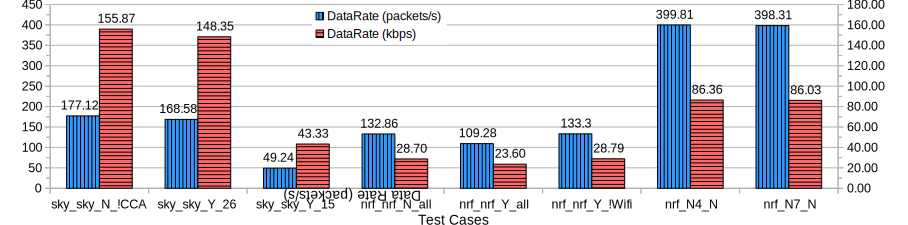
\includegraphics[width=\textwidth]{HT-dr}
\caption{Data Rate}
\label{fig:HT-dr}
\vspace{-6 pt}
\end{figure}

Note that in figure \ref{fig:HT-dr} there are two Y-axis representing the data rate in packets per second and kilobit per second. The link layer payload of 27 bytes and 110 byte was used for BLE and 802.15.4 respectively to calculate the data rate in kbps.

\begin{figure}[h]
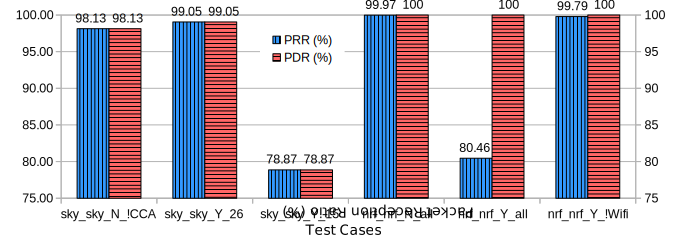
\includegraphics[width=\textwidth]{HT-r}
\caption{Reliability}
\label{fig:HT-r}
\vspace{-6 pt}
\end{figure}
The graph in figure \ref{fig:HT-r} has Y-axes from 75 to 100 \% for clearer representation of the \gls{pdr} and \gls{prr} \todo{Is this misleading?}. As mentioned in section \ref{6HTdesign} the reliability was calculate in BLE by logging the number of times the radio was switched on as this information was accessible from the SoftDevice. This allowed the calculation of \gls{prr} with one packet per connection event. Since the android devices can communicate multiple packets per connection event, the \gls{prr} could not be calculated. Hence, those test cases are not plotted.

\begin{figure}[h]
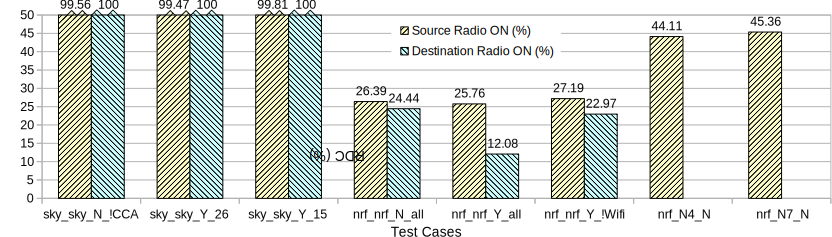
\includegraphics[width=\textwidth]{HT-ec}
\caption{Energy Consumption}
\label{fig:HT-ec}
\end{figure}

For a clearer representation of the graph, the y-axis in figure \ref{fig:HT-ec} is limited to 50\%. The break in the graph shows when Tmote-Sky uses \textasciitilde100\% of radio duty cycle. In all the tests with BLE the source node was the slave device sending the notifications, while the destination node was the master device receiving them.

There was no easy way of accessing the low level information of BLE \gls{rdc} on an Android device, so the energy consumption of these devices is not plotted. Moreover the energy consumption of such multi-purpose master device is less important than a single purpose slave device running on a meager battery.

\subsection{Analysis}
\paragraph{Data Rate}
The absolute data rate is higher in 802.15.4 than BLE although the number of packets transmitter per second is higher in BLE as seen in figure \ref{fig:HT-dr}. This is because of the higher packet size of 802.15.4 and the bit rate of transmission of BLE is four time the bit rate of 802.15.4 at 1 Mbps.

For 802.15.4 the peak data rate of 155.87 kbps is achieved when \gls{cca} is not used. The more practical approach of using \gls{cca} decreased in the data rate slightly to 148.35 kbps. When WiFi interference was introduced, most of the transmission slots were not utilized because of backing off by \gls{cca}. \hyperref[AppendixB]{Appendix B} shows that only 21\% of the transmission slots were used dropping the data rate considerably. With this 43.33  kbps data rate was achieved, which is higher than the data rate achieved by BLE communication between nodes of PCA10000 platform in any test case. Since 802.15.4's Null-RDC tries to send a packet as soon as possible, we can approximately calculate that the inference of WiFi traffic was not present 29.2\% of the time by taking the ratio of the data rate with and without WiFi interference (43.33/148.35).

The SoftDevice used to implement the central stack allows only one packet to be communicated per connection interval. With this the theoretical data rate that can be achieved can be found out by 

$\mbox{Data Rate  (packet/second)}=\frac{1}{\mbox{connection interval}}=\frac{1}{7.5ms}=133.33\:packet/second$

\vspace{15 pt}
$\mbox{Data Rate (kbps)}=\frac{\mbox{(bits per byte)}\times\mbox{(link layer payload in bytes)}}{\mbox{connection interval}}=\frac{8\times27}{7.5ms}=28.8\:kbps$
\vspace{10 pt}

The experimental results seen in figure \ref{fig:HT-dr} shows this is achieved accurately. When WiFi is introduced, the data rate drops from 28.7 kbps to 23.6 kbps, when all the channels are used. This is 82\% of the WiFi free data rate. Figure \ref{fig:Intf} shows that 10 out of the 37 data channels are interfered by WiFi traffic. This means that the data rate should reduce by (37-10)/37, which is about 73\% of the WiFi free data rate. The greater data rate achieved experimentally can be accounted to the fact that the WiFi traffic wasn't interfering 100\% of the time as inferred earlier. Considering that the 10 channels were interfered 29.2\% of the time as calculated, the data rate achievable can be calculated as $(0.292\times10/37 + 1\times27/37)\times28.8=24.1$ kbps which is closer to the achieved 23.6 kbps.

When the WiFi free channels were used the data rate recorded was close to the theoretical data rate predicted. There was no influence of the WiFi traffic at all for BLE communication in this case. This shows that when frequency hopping channel map is chosen to avoid the interference, there is no effect on the data rate.

Communication of the PCA10000 with a Nexus4/7 master device achieved a greater data rate of about 86 kbps or \textasciitilde400 packet/second. This is because the BLE stack in these Android devices support communication of multiple packets in a connection event, increasing the data rate achievable. With a connection interval of 7.5 ms, at an average there were around $(400\times7.5/1000)$ i.e. 3 packets of data received by the Android device per connection event.

\paragraph{Reliability}
In case of 802.15.4, the \gls{pdr} and \gls{prr} is same since it does not have any communication failure detection and retransmission mechanism. This is left to the upper layer to handle. The link layer just tries initiate communication when there is no external interference present with its \gls{cca}. Figure \ref{fig:HT-r} shows that the \gls{prr} achieved when \gls{cca} is switched off is 96.23\%. While it can be seen that without \gls{cca} the data-rate is higher, the reliability decreases. By using \gls{cca} in a WiFi free channel, the \gls{prr} increases to 99.55\%, which means that the \gls{cca} is effective in case of less interference. When there was heavy WiFi traffic in the same channel of communication, the \gls{cca} did work since only 21.11\% of the transmission slots were used. Of these transmissions the \gls{prr} was 84.7\%. This could happen when the interference starts after the carrier assessment, causing the packet to get corrupted. Here it can be seen that \gls{cca} of 802.15.4 has reduced effectiveness in case of heavy interference.

In case of \gls{ble}, figure \ref{fig:HT-r} shows that the \gls{pdr} is always 100\% since BLE employs a simple acknowledgment scheme to detect if the communication has not been successful so that the packet can be retransmitted. This ensures that the upper layers can safely assume that the link layer is completely reliable. Without WiFi interference \gls{prr} was about 99.64\%, which means that there were few retransmissions. With all the channels employed and with WiFi interference, the \gls{prr} reduced to 81.94\%. This number is not low because of the frequency hopping used by BLE, which ensures that interference in one frequency range only effects the communication happening over the channels in that frequency range. The other data channels can still keep the communication flow intact. This shows that the frequency hopping when used over the complete channel map helps in sustaining the communication when there is external interference. When only the WiFi free channels were employed, there was no influence of the WiFi interference on \gls{prr}, which was 99.95\%. This shows that when a master device has the capability of detecting external interference, it can adapt the frequency hopping channels so that there is negligible effect on the communication. Note that \gls{afh} can only help negate narrow band interference in the 2.4 GHz \gls{ism} band.

\paragraph{Energy Consumption}
As seen in figure \ref{fig:HT-ec}, the radio of Tmote-Sky nodes is used nearly 100\% the time in all the test cases of the \gls{ht} test suite. This shows that in 802.15.4 the data rate can be maximized, by choosing an appropriate \gls{rdc} layer like Null-RDC, although at the expense of energy consumption. 

When the test cases where the communication happened between PCA10000 node, the source node had \gls{rdc} of 25\% to 27\%. In the case \texttt{nrf\_nrf\_Y\_all} where the communication was affected by interference, the destination node had a 
\todo{redo tests for }

In case of communication with the Android devices, the source nodes had \gls{rdc} of 44\% to 45\%. This is higher because multiple packets were communicated per connection interval. With stacks supporting greater packets per connection interval, this number will increase, also increasing the throughput. This shows that when a master device can support communication of greater number packets per connection event, the data rate increases.

\section{\acrlong{rr} Test}

\subsection{Graphical Representation of Data Acquired}
\begin{figure}[h]
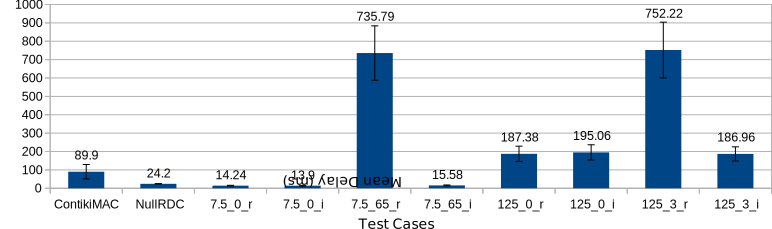
\includegraphics[width=\textwidth]{RR-l}
\caption{Latency}
\label{fig:RR-l}
\end{figure}

Figure \ref{fig:RR-l} shows the mean of the thousand measurement of latency in ms for different cases of the \gls{rr} test suite along with the standard deviation. 

\begin{figure}[h]
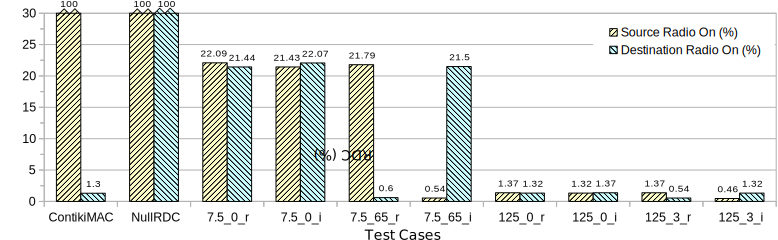
\includegraphics[width=\textwidth]{RR-ec}
\caption{Energy Consumption}
\label{fig:RR-ec}
\end{figure}

Figure \ref{fig:RR-ec} shows the energy consumption of the nodes in terms of the percentage of time the radio was switched on for the different cases of the \gls{rr} test suite. Similar to the graph for the \gls{ht} tests, this graph is limited to 30\% for clearer representation, especially of in test cases with low duty cycle.

In 802.15.4 the source and destination nodes can be identified based on who's sending and who's receiving. In case of BLE it is a bit more complicated since source and destination nodes change based on where the latency is being measured. In the tests with the master reading a packet from the slave, the master is the source while the slave is the destination. In tests with the slave sending an indication packet to the master and receiving an acknowledgment from it, the source and destination are inverted.

\subsection{Analysis}
\paragraph{Latency}
The latency measurement as seen from figure \ref{fig:RR-l} can vary in the order of magnitude among different tests. The least latency can be achieved using 802.15.4 when using Null-RDC, which is about 24 ms.  When using ContikiMAC, the average latency was about 90 ms, which can be attributed to the 125 ms interval with which the receiver wakes up. \todo{resposne in the same ack is happening, always possible?}.  \todo{update link layer config while running or is it hard coded?}

Based on the link layer configurations used for BLE, the latency varied from a minimum of about 14 ms to a maximum of about 750 ms. The provision in BLE's link layer for changing these configurations while in a connection is an advantage since the latency can be adapted according to the requirement. The configuration of the slave latency value determines if there is any difference in the latency experienced based on whether the communication happens with a read request or an indication. With slave latency as zero, the latency of the read and indication case is almost same, with the average latency being around 14 ms with 7.5 ms connection interval and 190 ms with a connection interval of 125 ms. With a non-zero slave latency value, the read-request from the master node (client in \gls{att}) has high latency since the slave node (server at \gls{att})will not react to the master at every connection interval as it is sleeping. With a slave latency value of 65, the master node can read a value from the slave node with a latency of about 736 ms, even with a connection interval of 7.5 ms. Similarly, with a slave latency of 3 and connection interval of 125 ms, the master will read a value from the slave with a latency of about 752 ms. When using indication to communicate data to a master, the latency can be low since the slave can decide to respond to the master when necessary communicate. With a 7.5 ms connection interval and slave latency of 65, the latency is about 15 ms, which is similar to the latency experience with zero slave latency. Similarly, an indication providing the master with data experiences a latency of 187 ms with a connection interval of 125 ms and slave latency of 3. This is almost equal to the latency experienced with zero slave latency. This shows that use of indication does not effect the latency experienced to send data to a master node in a connection with non-zero slave latency.

\paragraph{Energy Consumption}
The energy consumption of the 802.15.4 source and destination node is 100\% in terms of \gls{rdc} in case of Null-RDC. This is as expected because of the nature of Null-RDC implementation. In case of ContikiMAC, the source node has 100\% \gls{rdc} while the destination has 1.3\%. The source node has this high energy consumption because \todo{it is configured so. This is inline with the usual root node that has access to a wall socket and gathers data from the other nodes. It is the destination node which is battery operated and has to conserve energy.} 

In case of BLE, the energy consumption of the nodes which have to switch on their radio every 7.5 ms have the highest \gls{rdc} at around 21-22\%. This includes both the source and destination when the slave latency is zero and connection interval is 7.5 ms. In case the slave latency of 65 is used, the master has \gls{rdc} of around 21\%, while the slave has a \gls{rdc} of only 0.6\%. This is since the slave  can choose only to respond to the master every 66th connection interval and sleep the rest of the time, thereby creating an asymmetric architecture. Similarly when the connection interval is 125 ms and slave latency is zero, both master and slave node have 
approximately equal \gls{rdc} of 1.32 to 1.37\%. By using a slave latency of 3 and the same connection interval, the slave nodes were able to sleep for longer duration leading to the reduction of \gls{rdc} to around 0.6\%.
\chapter{Other Contributions}

\section{Firmware for demo application}



\section{Advertisement Logger}
\begin{figure}[h]
\includegraphics[width=\textwidth]{AdvLogger}
\caption{User Interface of Advertisement Logger}
\end{figure}
\chapter{Conclusion and Future Work} \label{9ConcFuture}
\section{Conclusion}

Contiki is ported to a BLE based platform, namely nrf51822 \gls{soc} based PCA10000. nrf51822 was chosen as the \gls{soc} to work with after comparing various commercially available \glspl{soc} in many criteria based on the formulated requirements of the platform. The port allowed all the basic peripherals of nrf51822 to be controlled by Contiki's libraries such as etimer, rtimer, serial-line and LEDs.  The radio was not included in the port since the radio was controlled by a SoftDevice binary for BLE operations and also since the Contiki radio \glspl{api} are not compatible with BLE operations. The test cases and the alarm application developed with the Contiki verify its working.

Two test suites were designed to compare four metrics of the link layer of BLE and 802.15.4, where 802.15.4 refers to use fof 802.15.4 physical layer and used of ContikMAC and Null-RDC \gls{mac} layers. The conducted test cases resulted in the following insights:

\begin{easylist}[itemize]
& The absolute data rate achievable with 802.15.4 is higher than BLE on the account of the greater link-layer payload size, which is 110 byte for 802.15.4 and 27 byte for BLE.
& The highest data rate achieved with 802.15.4 is when \gls{cca} wasn't used (155 kbps), followed by communicating with a channel not overlapping with external interference using \gls{cca} (148 kbps) and the case where the channel was interfered with WiFi signals was where the data rate recorded was least for 802.15.4 (61 kbps).
& In case of BLE, the highest data rate was recorded when communicating with an Android device (86 kbps), since the master device allowed multiple packets to be communicated in a connection interval. The data rate achieved between PCA10000 nodes was in-line with the theoretically calculated data rate when there was no external interference and when WiFi free channel map was used (29 kbps). Seen here is that if \gls{afh} is implemented, there is no degradation in the data rate in the presence of external interference. When there was WiFi interference and the complete channel map was used, the data rate dropped to 23 kbps.
& The data rate achieved in BLE communication depends highly on the stack, which limits the deciding parameters of connection interval and packets communicated consistently in each connection interval.
& \gls{cca} operation in 802.15.4 has greater efficiency in case of low external interference (99\% \gls{prr}) as compared to high external interference  (79\% \gls{prr}).
& The acknowledgment scheme of BLE does result in 100\% \gls{pdr} for the layers above the link layer in all cases. The \gls{prr} with BLE is greater than 99\% when there was no external interference and when WiFi free channel map was used. 80\% \gls{prr} was achieved when all the channel map was used with external interference, which shows that narrow band interference affects only a small portion of the communication.
& When one packet was communicated per connection interval, the \gls{rdc} was between 26 and 29\%. This value increased to about 44\% when an average of 3 packets were communicated per connection event.
& Null-RDC and ContikiMAC achieved a latency of 24 ms and 90 ms respectively for a read-response operation. ContikiMAC achieved this latency with the destination node achieving only 1.3\% \gls{rdc}.
& The latency measurement with BLE nodes ranged from 14 ms to 750 ms depending on the configuration. The variation of the symmetric of the connection can illustrated in the case where the slave devices energy consumption drops drastically without change in the latency when using indication packets. This can result in cases where 14 ms latency can be achieved by a master and slave node consuming only 21.5\% and 0.54\% radio on time.
& Use cases where low latency is required for data to communicated from the master to slave, the slave latency value used must be close to zero. In other cases large slave latency values can be used. The provision for dynamic update of the link layer parameters of a BLE connection is useful in optimizing these parameters for different scenarios.

\end{easylist}

\section{Future Work}

The lack of availability of a complete and open-source BLE stack is one of the major inhibiting factors faced by researchers working with \gls{ble}. This results in little or no flexibility in developing the test setup as needed for the research projects. Contiki is a mature platform under active development for \gls{iot} projects. This thesis project can provide a start to active development of an open-source BLE stack and support for greater number of BLE sed platforms in Contiki.


\printbibliography[title={References}]

\appendix
\chapter{Appendix | \gls{ble} \gls{soc} Comparison} \label{AppendixA}
The dense table in the next page compares many different parameters of the \gls{ble} \glspl{soc} available. This table was compiled in the first half of 2014. Because of the high pace at which the industry around \gls{ble} is progressing, many details here might not be accurate as time progresses.

The legend for the table is

\vspace{10pt}
NA \hspace{10pt}: The information is not available

- \hspace{22pt}: The feature is not available



\includepdf[pagecommand={\begin{tikzpicture} [remember picture,overlay] \node at (7.4,-17) {}; \end{tikzpicture}},page=1]{BLE_SoCs.pdf}

\end{document}          
